The new scenario we have to consider is the one in which only the conversion rates of the customers are unknown. Also, the features of our customers are unknown, so our website is not able to distinguish one from another. \\
To solve the problem, two bandit algorithms have been developed: UCB-1 (Upper Confidence Bound) and TS (Thompson Sampling).
Both select every day the super arm to pull by estimating the conversion rates, with their parameters. After that, they run a Montecarlo simulation for each combination of arms, in order to determine the best super arm (the one that returns the highest reward estimated).\\
The super arm selected is pulled into the environment to collect the actual reward and the learners' parameters can be updated.\\
Since the learners are not able to distinguish the different types of customers, the conversion rates estimated each round by the learner are set equal for every type of customer.\\
The number of daily interactions (customers that visit the e-commerce) is fixed to 100 and the time horizon (the number of days of exploration of the algorithm) to 300. The number of iterations is set to 5 (the number of times the algorithms are executed).

\subsection{UCB-1}
Upper Confidence Bound is a deterministic algorithm that associates an upper confidence bound to every arm, providing an optimistic estimation of the reward.
The steps are the following:
\begin{enumerate}
    \item Initially the means and the upper confidence bounds of each arm (price) for each product are set to zero and infinite respectively \[ means=
    \begin{bmatrix}
            0 & 0 & 0 & 0\\
            0 & 0 & 0 & 0\\
            0 & 0 & 0 & 0\\
            0 & 0 & 0 & 0\\
            0 & 0 & 0 & 0
    \end{bmatrix}upperBound=
    \begin{bmatrix}
            \infty & \infty & \infty & \infty\\
            \infty & \infty & \infty & \infty\\
            \infty & \infty & \infty & \infty\\
            \infty & \infty & \infty & \infty\\
            \infty & \infty & \infty & \infty
    \end{bmatrix}
    \]
    \item Estimate the conversion rates by the sum of the mean and the upper confidence bound of each arm\begin{minted}[breaklines]{python}
        def estimate_conversion_rates(self):
                return self.means + self.upper_bounds
        \end{minted}
    \item Select the super arm that returns the highest reward from the MC simulation and use it to interact with the environment
    \item Update the mean parameters of the pulled arm as:\begin{equation}
            mean[p,a] = \frac{mean[p,a] * seen[p,a] + bought[p]}{tot\_seen[p,a]}
        \end{equation}Where:
        \begin{itemize}
            \item mean[p,a] is the actual mean of the product {\bf p} with price {\bf a}
            \item seen[p,a] is the number of times the product {\bf p} with price {\bf a} has been seen until the day before
            \item bought[p] is the number of times the product {\bf p} has been bought from day zero untill now
            \item tot\_seen[p,a] is the number of times the product {\bf p} with price {\bf a} has been seen from day zero untill now (so is seen[p,a] plus the number of times this product has been seen today)
        \end{itemize}
    \item Update the upper confidence bound parameters of the arm pulled as according to the observations of the environment:
        \begin{equation}
            upper\_bound[p,a] = \sqrt{\frac{2 * \log (tot\_samples)}{seen[p,a]}}
        \end{equation}Where:
        \begin{itemize}
            \item tot\_samples is the total number of times the product {\bf p} has been seen untill now
            \item seen[p,a] is the number of times the product {\bf p} with price {\bf a} has been seen  untill now
        \end{itemize}
    \item Repeat from step 2 until the end of the interactions (300 days)
\end{enumerate}
\subsubsection{Results}
Even if the algorithm converges to the optimal arm at the beginning of the process, someday it will change the choice of the super arm to pull. This happens because each time an arm is pulled its bound is reduced, whereas at each time step, the upper bound of all arms logarithmically increases, so at some point, the ones less selected will have a higher bound. A bigger bound leads to a higher conversion rate. Due to this reason, the learner will try new super arms that were not pulled for a long time.
\begin{figure}[ht]
    \begin{center}
    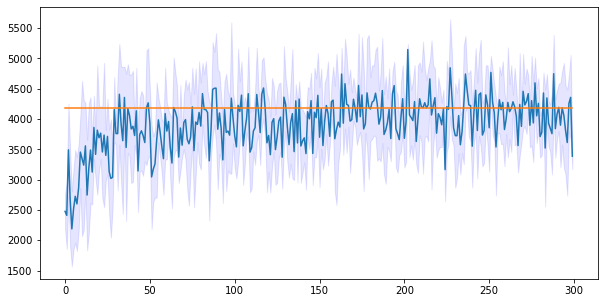
\includegraphics[width=0.5\textwidth]{img/ucb3.png}
    \caption{UCB Reward}
    \label{fig:reward31}
    \end{center}
\end{figure}
\begin{multicols}{2}
    \begin{figure}[H]
        \begin{center}
        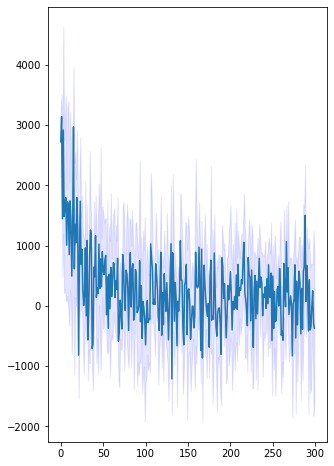
\includegraphics[width=0.5\textwidth]{img/ucb3_regret.png}
        \caption{UCB Regret}
        \label{fig:regret31}
        \end{center}
    \end{figure}
    \columnbreak
    \begin{figure}[H]
        \begin{center}
        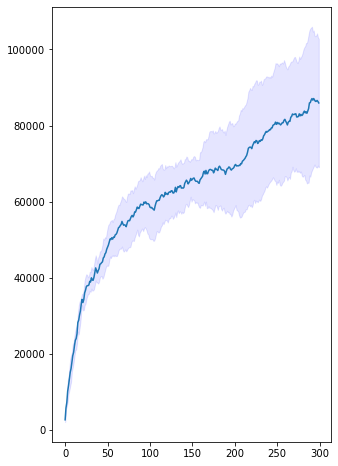
\includegraphics[width=0.5\textwidth]{img/ucb3_cum_reg.png}
        \caption{UCB Cumulative regret}
        \label{fig:cum_reg31}
        \end{center}
    \end{figure}
\end{multicols}


\subsection{TS}
Thompson Sampling is a stochastic algorithm that sets a prior on the expected value for every arm, and selects the arm with the best sample, according to the updated parameters. Those parameters are called Beta parameters and take account of the number of successes ($\alpha$) and failures ($\beta$). The sum of the two parameters is equal to the number of times the arm has been pulled.\\
Since we are dealing with a combinatorial problem, for each arm, we draw a sample from their conversion rate prior distribution and use those samples to evaluate the value of each super arm.\\
The steps are the following:
\begin{enumerate}
    \item Set all the $\alpha$ and $\beta$ parameters equal to one. \[\begin{bmatrix}
    \begin{bmatrix}
        1 & 1\\
        1 & 1\\
        1 & 1\\
        1 & 1\\
    \end{bmatrix}
    \begin{bmatrix}
        1 & 1\\
        1 & 1\\
        1 & 1\\
        1 & 1\\
    \end{bmatrix}
    \begin{bmatrix}
        1 & 1\\
        1 & 1\\
        1 & 1\\
        1 & 1\\
    \end{bmatrix}
    \begin{bmatrix}
        1 & 1\\
        1 & 1\\
        1 & 1\\
        1 & 1\\
    \end{bmatrix}
    \begin{bmatrix}
        1 & 1\\
        1 & 1\\
        1 & 1\\
        1 & 1\\
    \end{bmatrix}
    \begin{bmatrix}
        1 & 1\\
        1 & 1\\
        1 & 1\\
        1 & 1\\
    \end{bmatrix}
    \end{bmatrix} \]
    \item Estimate the conversion rate by drawing a sample from a Beta distribution with $\alpha$ and $\beta$ parameters \begin{minted}[breaklines]{python}
        def estimate_conversion_rates(self):
            return np.random.beta(a=self.beta_parameters[:, :, 0], b=self.beta_parameters[:, :, 1])
        \end{minted}
    \item Select the super arm that returns the highest reward from the MC simulation and use it to interact with the environment.
    \item Update the $\alpha$ and $\beta$ parameters according to the observations of the environment:\\
        $\alpha$[p, a] = $\alpha$[p, a] + bought[p]\\\\
        $\beta$[p, a] = $\beta$[p, a] + seen[p] - bought[p]
    \begin{itemize}
        \item $\alpha[p, a]$ is the alpha parameter for the product {\bf p} with the price {\bf a}
        \item $\beta[p, a]$ is the beta parameter for the product {\bf p} with the price {\bf a}
        \item bought[p] is the number of times the product {\bf p} has been bought untill now
        \item seen[p] is the number of times the product {\bf p} has been visualized by the customers
    \end{itemize}
    \item Repeat from step 2 until the end of the interaction (300 days)
\end{enumerate}
\subsubsection{Results}
As we can see below the algorithm converges to the optimal super arm very quickly, so the regret goes to zero in the very first days. This is what we expected when there is a prior information that influences the choice of an arm.
\begin{figure}[ht]
    \begin{center}
    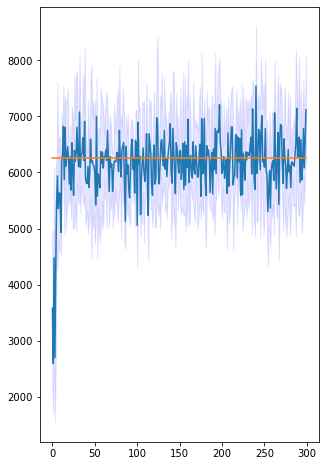
\includegraphics[width=0.5\textwidth]{img/TS3.png}
    \caption{TS Reward}
    \label{fig:reward32}
    \end{center}
\end{figure}
\begin{multicols}{2}
    \begin{figure}[H]
        \begin{center}
        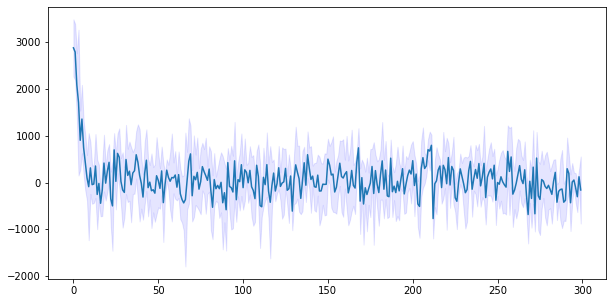
\includegraphics[width=0.5\textwidth]{img/TS3_regret.png}
        \caption{TS Regret}
        \label{fig:regret32}
        \end{center}
    \end{figure}
    \columnbreak
    \begin{figure}[H]
        \begin{center}
        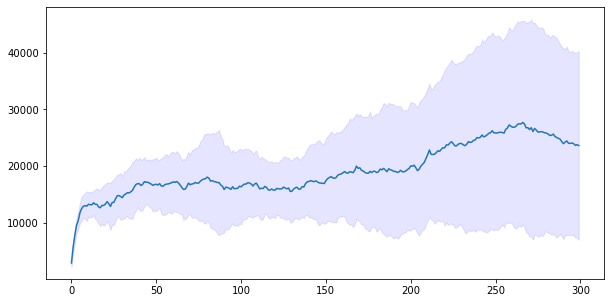
\includegraphics[width=0.5\textwidth]{img/TS3_cum_reg.png}
        \caption{TS Cumulative regret}
        \label{fig:cum_reg32}
        \end{center}
    \end{figure}
\end{multicols}
